\documentclass{article}
\usepackage[margin=1.1in]{geometry}
\usepackage{graphicx}
\usepackage{amsmath}
\usepackage{hyperref}
\usepackage{booktabs} % For professional tables

% Packages for code and output boxes
\usepackage{xcolor}
\usepackage{listings}
\usepackage{tcolorbox}
\tcbuselibrary{listings, skins, breakable} % <--- Added 'breakable' here!

% Define the style for C++ syntax highlighting
\lstdefinestyle{cppstyle}{
    language=C++,
    basicstyle=\ttfamily\scriptsize, 
    keywordstyle=\color{blue!80!black}\bfseries,
    stringstyle=\color{red!70!black},
    commentstyle=\color{green!50!black}\itshape,
    showstringspaces=false,
    numbers=left,
    numberstyle=\tiny\color{gray},
    numbersep=3.5pt, % Adjust this value to move the line numbers left or right   breaklines=true,
    tabsize=4
}

% Create the Code Box environment
\newtcblisting{codebox}[1]{
    arc=3mm,
    boxrule=1pt,
    colback=blue!5!white,
    colframe=blue!75!black,
    title={\textbf{#1}},
    listing only,
    listing style=cppstyle,
    breakable % <--- Added this to allow page breaks!
}

% Create the Output Box environment
\newtcolorbox{outputbox}[1]{
    arc=3mm,
    boxrule=1pt,
    colback=black!85!white,
    colframe=black,
    coltext=white,
    title={\textbf{#1}},
    fontupper=\ttfamily\scriptsize,
    left=2mm, right=2mm, top=2mm, bottom=2mm,
    fontupper=\ttfamily\scriptsize\obeylines, % <--- Added \obeylines here!
    breakable % <--- Added this to allow page breaks!
}

\title{PHYS 551: Homework 1}
\author{Your Name Here}
\date{February 24, 2026}

\begin{document}


% =======================================================
% COVER PAGE
% =======================================================

% =======================================================
% MODERN COVER PAGE
% =======================================================

\begin{titlepage}
\begin{center}

% Top 

\includegraphics[width=0.55\textwidth]{images/ozu.png}\\[2cm]

\rule{\linewidth}{0.5mm}\\[0.4cm]

% Title
{ \LARGE 
  \textbf{PHYS551: Advanced Monte Carlo Methods}\\[0.4cm]
  \emph{Homework 1}\\[0.4cm]
}
\rule{\linewidth}{0.5mm}\\[0.4cm]

\hfill
\hfill

% Author
\linewidth=0.8\textwidth

	\begin{minipage}{0.4\textwidth}
		\begin{flushleft} \large
			\emph{Student:}\\
			Ömer Faruk \textsc{Avcı} % Your name here
		\end{flushleft}
	\end{minipage}
	~
	\begin{minipage}{0.5\textwidth} % Made slightly wider to fit long titles
		\begin{flushright} \large
			\emph{Instructor:}\\
			Prof. Taylan \textsc{Akdo\u{g}an}\\[0.1cm]

		\end{flushright}
	\end{minipage}
	


\vfill

%\textsc{\Large Cyprus University of Technology}\\[0.4cm]
\textsc{\large Department of Electrical and Electronics Engineering}\\[0.4cm]




% Bottom
{\large \today}
 
\end{center}
\end{titlepage}

% =======================================================
% START OF CONTENT
% =======================================================


% =======================================================
% START OF CONTENT
% =======================================================



\section*{Disclosures and References}
\textbf{AI Usage Disclosure:} In accordance with the course policy, I would like to declare the extent of AI assistance used in this assignment:
\begin{itemize}
    \item \textbf{Code Implementation:} I personally implemented the core physics algorithms, including the \texttt{estimate\_pi} function for Problem 2 and the \texttt{single\_random\_walk} / \texttt{simulate\_M\_walks} functions for Problem 3. AI tools were used to assist in writing the wrapper loops for ensemble averaging, generating the plotting scripts, and refining code comments.
    \item \textbf{Report Generation:} AI assistance was used to generate the LaTeX structure for this report, specifically for creating the "paper-style" layout, formatting the code/terminal output boxes, and refining the phrasing of the mathematical derivations.
\end{itemize}
\vspace{0.5cm}
\hrule
\vspace{0.5cm}
\textbf{External References:} 
\begin{itemize}
    \item The random number generation in my C++ code was implemented using documentation from \href{https://en.cppreference.com/w/cpp/numeric/random/uniform_real_distribution}{cppreference.com (std::uniform\_real\_distribution)}.
\end{itemize}
\vspace{0.5cm}
\hrule
\vspace{0.5cm}
\textbf{Technical Note:} Detailed instructions for compiling the source code on both Linux and macOS, including how to handle the \texttt{matplotlib-cpp} dependency and how to toggle specific simulation tasks, are provided in \textbf{Appendix C}.



% ==========================================
% PROBLEM 1
% ==========================================
\section*{Problem 1: Preparation}


\begin{figure}[h]
    \centering
    
\includegraphics[width=0.95\textwidth]{images/problem_1_figure.png}
    \caption{Screenshot of my IDE running the "Hello Monte Carlo" script and a simple plot.}
\end{figure}

\newpage
% ==========================================
% PROBLEM 2
% ==========================================
\section*{Problem 2: The Cost of Precision (Estimating $\pi$)}

\subsection*{1. Derivations}
The Monte Carlo "Darts in a Square" method relies on the geometric probability of a point falling within a specific region. We define a square domain with $x \in$ and $y \in$, which yields a total area of:
\begin{equation}
    A_{\text{square}} = 2 \times 2 = 4
\end{equation}
An inscribed circle of radius $r = 1$ has an area of:
\begin{equation}
    A_{\text{circle}} = \pi r^2 = \pi (1)^2 = \pi
\end{equation}
If $N$ points are sampled uniformly across the square domain, the probability $P$ of any single point falling inside the circle is the ratio of the areas. Therefore, the expected number of points inside the circle, $N_{\text{inside}}$, is:
\begin{equation}
    \frac{N_{\text{inside}}}{N} \approx P = \frac{A_{\text{circle}}}{A_{\text{square}}} = \frac{\pi}{4} \implies \pi \approx 4 \times \frac{N_{\text{inside}}}{N}
\end{equation}
Because this is a stochastic process modeled by a binomial distribution (a point is either inside or outside), the standard error of the mean scales inversely with the square root of the number of trials. Thus, the theoretical standard error scales as:
\begin{equation}
    \text{Error} \propto \frac{1}{\sqrt{N}} = O(N^{-0.5})
\end{equation}
Taking the base-10 logarithm of both sides yields a linear relationship:
\begin{equation}
    \log_{10}(\text{Error}) \approx -0.5 \log_{10}(N) + C
\end{equation}
where $-0.5$ is the theoretical slope of the Log-Log plot.

\subsection*{2. Analysis \& Implementation}
To empirically verify the $1/\sqrt{N}$ scaling law, a simulation was implemented in \textbf{C++}. This language was selected for its high performance, which is essential for handling large sample sizes ($N=10^7$) within a reasonable execution time.

For the random number generation, the simulation utilizes the C++11 \texttt{<random>} library rather than the legacy \texttt{rand()} function. Specifically, the \textbf{Mersenne Twister 19937} engine (\texttt{std::mt19937}) was chosen. This generator provides a period of $2^{19937}-1$, which is orders of magnitude larger than the total samples used in this experiment, ensuring that the sequence does not repeat or exhibit significant correlations during the simulation. This engine drives a \texttt{std::uniform\_real\_distribution} to produce high-precision floating-point values uniformly distributed in the domain $[-1, 1]$.

Because a single Monte Carlo realization is subject to high statistical variance, the simulation was repeated $10$ times for each $N$. The average absolute error was calculated over $k=10$ runs:
\begin{equation}
    \text{Error}_N = \frac{1}{10} \sum_{k=1}^{10} |\hat{\pi}_{N,k} - \pi_{\text{true}}|
\end{equation}
The full C++ implementation is displayed below (output is provided in Appendix A):
\newpage
\begin{codebox}{C++ Source Code: Problem 2 Complete Implementation}
#include <iostream>
#include <random>
#include <cmath> 
#include "matplotlibcpp.h"

std::random_device rd; // Random device for seeding
std::mt19937 gen(rd()); // Mersenne Twister random number generator
std::uniform_real_distribution<> square_dist(-1.0, 1.0); // Distribution for x and y coordinates
std::uniform_real_distribution<> angle_dist(0.0, 2.0 * M_PI); // Distribution for random walk angles

/* 
 * -----------------------------------------------------------------
 * Problem 2: The Cost of Precision (Estimating Pi)
 * -----------------------------------------------------------------
 */

// Core Monte Carlo Function: "Darts in a Square"
// Estimates Pi by placing a circle of radius 1 inside a 2x2 square.
double estimate_pi(int N){
    
   

    int inside = 0; // Counter for points that fall inside the inscribed circle

    for(int i = 0; i < N; i++){
        double x = square_dist(gen); // x coordinate between -1 and 1
        double y = square_dist(gen); // y coordinate between -1 and 1

        // Check if the point falls inside the circle of radius r=1
        // Equation of circle: x^2 + y^2 <= r^2
        if(x*x + y*y <= 1.0){
            inside++;
        }
    }

    // Ratio of areas: (Area of Circle) / (Area of Square) = (pi * r^2) / (2r)^2 = pi / 4
    // Therefore, Pi is estimated as 4 * (Points Inside / Total Points N)
    return 4.0 * inside / N;
}


// -----------------------------------------------------------------
// Part (a): 
// Takes an array of N values, performs one simulation per N, and prints the result.
// -----------------------------------------------------------------
void run_problem_2_a(int N[], int size){
    for(int i = 0; i < size; i++){
        double pi_estimate = estimate_pi(N[i]);
        std::cout << "N: " << N[i] << " Estimated Pi: " << pi_estimate << std::endl;
    }
}


// -----------------------------------------------------------------
// Part (b):
// This function runs the simulation 'runs' times for each N and averages the estimates.
// -----------------------------------------------------------------
void run_problem_2_b(int N_values[], int size, int runs) {

    for (int i = 0; i < size; i++) {
        int N = N_values[i];
        double sum_pi = 0.0;

        std::cout << "========================" << std::endl;
        std::cout << "N = " << N << std::endl;

        for (int k = 0; k < runs; k++) {
            double pi_estimate = estimate_pi(N);

            std::cout << "Run " << k+1
                      << " | Pi Estimate: "
                      << pi_estimate << std::endl;

            sum_pi += pi_estimate; // Accumulate estimates for averaging
        }

        double average_pi = sum_pi / runs;

        std::cout << "Average Pi for N = "
                  << N << " : "
                  << average_pi << std::endl;
    }
}


// -----------------------------------------------------------------
// Part (c):
// Runs the simulation 10 times for each N, calculates the absolute error
// against the true value of Pi (M_PI), and finds the average error.
// -----------------------------------------------------------------
void run_problem_2_c(int N_values[], int size) {
    const int runs = 10; // As required by the homework prompt

    for (int i = 0; i < size; i++) {
        int N = N_values[i];
        double error_sum = 0.0;

        std::cout << "==============================" << std::endl;
        std::cout << "N = " << N << std::endl;

        for (int k = 0; k < runs; k++) {
            double pi_estimate = estimate_pi(N);
            
            // Calculate absolute error: |pi_estimate - pi_true|
            double error = std::abs(pi_estimate - M_PI);

            std::cout << "Run " << k+1
                      << " | Pi Estimate: " << pi_estimate
                      << " | Absolute Error: " << error
                      << std::endl;

            error_sum += error; // Accumulate errors
        }

        // Calculate the average absolute error for the current N
        double average_error = error_sum / runs;

        std::cout << "Average Absolute Error for N = "
                  << N << " : "
                  << average_error << std::endl;
    }
}

void run_problem_2(){
    // Define the sample sizes as requested in the assignment: 10^1 to 10^7
    int N[] =  {10, 100, 1000, 10000, 100000, 1000000, 10000000};
    int size = sizeof(N) / sizeof(N[0]); // Dynamically calculate array size
    
    // Run Problem 2a
    std::cout << "\nRunning Problem 2a: Single Simulation for Each N" << std::endl;
    run_problem_2_a(N, size);
    
    // Run Problem 2b 
    std::cout << "\nRunning Problem 2b: 10 Simulations for Each N and Averaging" << std::endl;
    int runs = 10;
    run_problem_2_b(N, size, runs);
    
    // Run Problem 2c
    std::cout << "\nRunning Problem 2c: Error Analysis" << std::endl;
    run_problem_2_c(N, size);
}

\end{codebox}
\newpage
\subsection*{3. Experimental Results \& Discussion}
Using the terminal output generated by the C++ simulation (refer to Appendix A), the average absolute error for each sample size $N$ was tabulated. To visualize the power-law scaling, a Python script was used to plot these values on a Log-Log scale (the full Python script is provided in \textbf{Appendix B}).

\begin{table}[h]
    \centering
    \caption{Experimental Error Analysis ($k=10$ runs per $N$)}
    \begin{tabular}{@{}llcc@{}}
        \toprule
        $N$ (Samples) & $\log_{10}(N)$ & Average Absolute Error & $\log_{10}(\text{Error})$ \\ \midrule
        $10^1$        & 1              & 0.355044              & $-0.4497$                 \\
        $10^2$        & 2              & 0.115681              & $-0.9367$                 \\
        $10^3$        & 3              & 0.044163              & $-1.3549$                 \\
        $10^4$        & 4              & 0.010280              & $-1.9880$                 \\
        $10^5$        & 5              & 0.004530              & $-2.3439$                 \\
        $10^6$        & 6              & 0.001380              & $-2.8601$                 \\
        $10^7$        & 7              & 0.000419              & $-3.3779$                 \\ \bottomrule
    \end{tabular}
\end{table}

\textbf{Discussion:} The experimental data strongly corroborates the theoretical predictions of Monte Carlo error scaling. As shown in the table, when $\log_{10}(N)$ increases by $1$ (representing a $10\times$ increase in sample size), the $\log_{10}(\text{Error})$ decreases by approximately $0.5$. 

This trend is visualized in Figure 1, where the experimental data points form a linear trend with a slope of roughly $-0.5$. This matches the $O(N^{-1/2})$ theoretical scaling law derived in class. Mathematically, this illustrates the "Cost of Precision": to reduce the standard error by a factor of 10, the computational workload ($N$) must be increased by a factor of 100.

\begin{figure}[h]
    \centering
    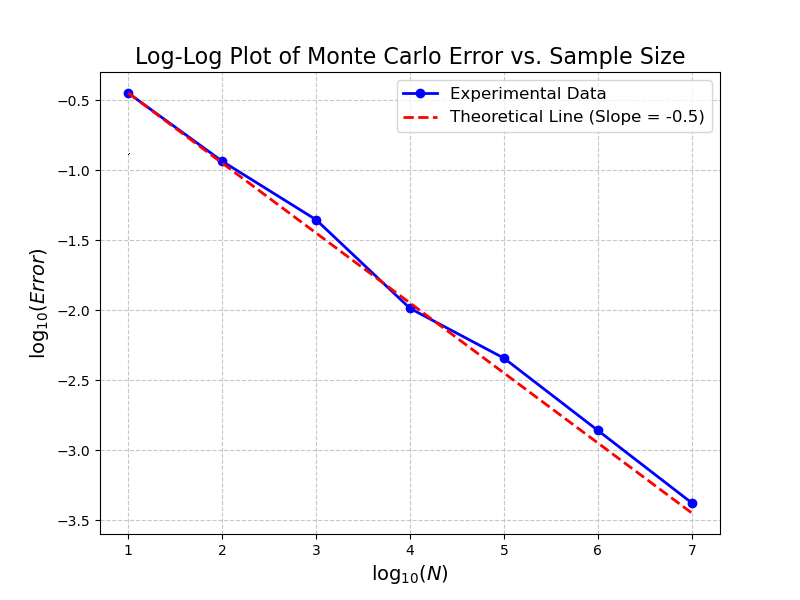
\includegraphics[width=0.8\textwidth]{images/problem_2_figure.png} 
    \caption{Log-Log plot of Average Absolute Error vs. $N$ }
    \label{fig:mc_error}
\end{figure}

\newpage

% ==========================================
% PROBLEM 3
% ==========================================
\section*{Problem 3: The "Drunkard's Walk" (2D Random Walk)}

\subsection*{1. Derivations}
A 2D random walk consists of $T$ steps of length $L=1$. The position vector after $T$ steps is the vector sum of individual steps $\vec{r}_i$:
\begin{equation}
    \vec{R}_T = \sum_{i=1}^{T} \vec{r}_i
\end{equation}
The mean squared distance from the origin is given by the ensemble average of the dot product $\vec{R}_T \cdot \vec{R}_T$:
\begin{equation}
    \langle R^2 \rangle = \left\langle \left( \sum_{i=1}^{T} \vec{r}_i \right) \cdot \left( \sum_{j=1}^{T} \vec{r}_j \right) \right\rangle = \sum_{i=1}^{T} \langle r_i^2 \rangle + \sum_{i \neq j} \langle \vec{r}_i \cdot \vec{r}_j \rangle
\end{equation}
Since the step directions are random and uncorrelated (isotropic), the cross-terms $\langle \vec{r}_i \cdot \vec{r}_j \rangle$ average to zero. Since each step has length $L=1$, $\langle r_i^2 \rangle = 1$. Thus:
\begin{equation}
    \langle R^2 \rangle = \sum_{i=1}^{T} 1 = T \implies D_{\text{rms}} = \sqrt{\langle R^2 \rangle} = \sqrt{T}
\end{equation}
For $T=1000$ steps, the theoretical prediction is $D_{\text{rms}} = \sqrt{1000} \approx 31.622$.

\subsection*{2. Analysis \& Implementation}
The simulation tracks a particle starting at $(0,0)$. At each step, a random angle $\theta \sim U[0, 2\pi)$ is generated using \texttt{std::uniform\_real\_distribution}, and the position is updated:
\begin{equation}
    x_{t+1} = x_t + \cos(\theta), \quad y_{t+1} = y_t + \sin(\theta)
\end{equation}
Two experiments were performed:
\begin{itemize}
    \item \textbf{Single Realization:} One walker taking $T=1000$ steps to visualize the trajectory.
    \item \textbf{Ensemble Average:} $M=1000$ independent walkers (each $T=1000$) to calculate the Root Mean Square (RMS) distance:
    \begin{equation}
        D_{\text{rms}} = \sqrt{\frac{1}{M} \sum_{i=1}^{M} (x_i^2 + y_i^2)}
    \end{equation}
\end{itemize}

\begin{codebox}{C++ Source Code: Problem 3 Complete Implementation}#include <iostream>
#include <random>
#include <cmath> 
#include "matplotlibcpp.h"

std::random_device rd; // Random device for seeding
std::mt19937 gen(rd()); // Mersenne Twister random number generator
std::uniform_real_distribution<> square_dist(-1.0, 1.0); // Distribution for x and y coordinates
std::uniform_real_distribution<> angle_dist(0.0, 2.0 * M_PI); // Distribution for random walk angles

/* 
 * -----------------------------------------------------------------
 * Problem 3: The “Drunkard’s Walk” (2D Random Walk)
 * -----------------------------------------------------------------
 */


// Core Random Walk Function: Simulates a single random walk of 'steps' steps and 
// returns the squared distance from the origin.
double single_random_walk(int steps) {

    double x = 0.0;
    double y = 0.0;

    for (int i = 0; i < steps; i++) {
        double angle = angle_dist(gen);
        x += std::cos(angle);
        y += std::sin(angle);
    }

    return x*x + y*y;  // return R^2
}

// Simulates 'walks' number of random walks, each with 'steps' steps,
// and returns the root mean square distance from the origin.
double simulate_M_walks(int steps, int walks) {

    double r2_sum = 0.0; 

    for (int i = 0; i < walks; i++) {
        r2_sum += single_random_walk(steps);
    }

    double mean_r2 = r2_sum / walks;
    double rms_distance = std::sqrt(mean_r2);

    return rms_distance;
}


// Even though single_random_walk function is defined, since the problem 3.a asks for plotting a single random walk,
// I will implement the plotting logic directly in run_problem_3_a function.
void run_problem_3_a(int steps) {
    double x = 0.0;
    double y = 0.0;
    
    std::vector<double> x_coords, y_coords;
    x_coords.push_back(x);
    y_coords.push_back(y);

    for (int i = 0; i < steps; i++) {
        double angle = angle_dist(gen);
        x += std::cos(angle);
        y += std::sin(angle);
        x_coords.push_back(x);
        y_coords.push_back(y);
    }
    
    matplotlibcpp::figure();
    matplotlibcpp::plot(x_coords, y_coords, {{"color", "blue"}, {"linestyle", "-"}, {"label", "Path"}});
    matplotlibcpp::plot({x_coords[0]}, {y_coords[0]}, {{"color", "green"}, {"marker", "o"}, {"label", "Start"}, {"markersize", "8"}});
    matplotlibcpp::plot({x_coords.back()}, {y_coords.back()}, {{"color", "red"}, {"marker", "^"}, {"label", "End"}, {"markersize", "8"}});
    matplotlibcpp::xlabel("x");
    matplotlibcpp::ylabel("y");
    matplotlibcpp::title("2D Random Walk (Drunkard's Walk)");
    matplotlibcpp::legend();
    matplotlibcpp::grid(true);
    matplotlibcpp::show();

    double r = std::sqrt(x*x + y*y);
    std::cout << "Final position: (" << x << ", " << y << ")" << std::endl;
    std::cout << "Distance from origin: " << r << std::endl;
}


// This function simulates 'walks' number of random walks, each with 'steps' steps, 
// and computes the root mean square distance from the origin.
void run_problem_3_b_c(int steps, int walks) {
    double rms_distance = simulate_M_walks(steps, walks);
    std::cout << "RMS Distance from Origin after " << steps 
              << " steps and " << walks 
              << " walks: " << rms_distance << std::endl;
}

void run_problem_3() {

    int steps = 1000;
    int walks = 1000;
    std::cout << "\nRunning Problem 3a: Single Random Walk Simulation with 1000 Steps" << std::endl;
    run_problem_3_a(steps); // Simulate and plot a single random walk with 1000 steps
    std::cout << "\nRunning Problem 3b/c: Simulate 1000 Random Walks and Compute RMS Distance" << std::endl;
    run_problem_3_b_c(steps, walks); // Simulate 1000 random walks and compute RMS distance
}
\end{codebox}


\subsection*{3. Results \& Discussion}
The trajectory of a single random walker (Task a) is shown in Figure 3. The path exhibits characteristic diffusive behavior, moving away from the origin in a jagged, non-linear path.

For the ensemble average (Task b/c), the RMS distance was calculated over $M=1000$ independent simulations.

\begin{outputbox}{Terminal Output: Problem 3 Results}
==========================
Running Problem 3: The Drunkard's Walk
==========================

Running Problem 3a: Single Random Walk Simulation with 1000 Steps
Final position: (4.82109, -12.2965)
Distance from origin: 13.2078

Running Problem 3b/c: Simulate 1000 Random Walks and Compute RMS Distance
RMS Distance from Origin after 1000 steps and 1000 walks: 31.3572
\end{outputbox}

\textbf{Discussion:} The simulation yielded an RMS distance of $\mathbf{31.3572}$. 
Comparing this to the theoretical prediction derived from the diffusion equation:
\begin{equation}
    D_{\text{theory}} \approx \sqrt{T} = \sqrt{1000} \approx 31.6228
\end{equation}
The experimental result is extremely close to the theoretical value, with a relative error of approximately $0.8\%$. This confirms that the particle's displacement scales with the square root of time (steps), which is the fundamental signature of a diffusive process.

\begin{figure}[h]
    \centering
    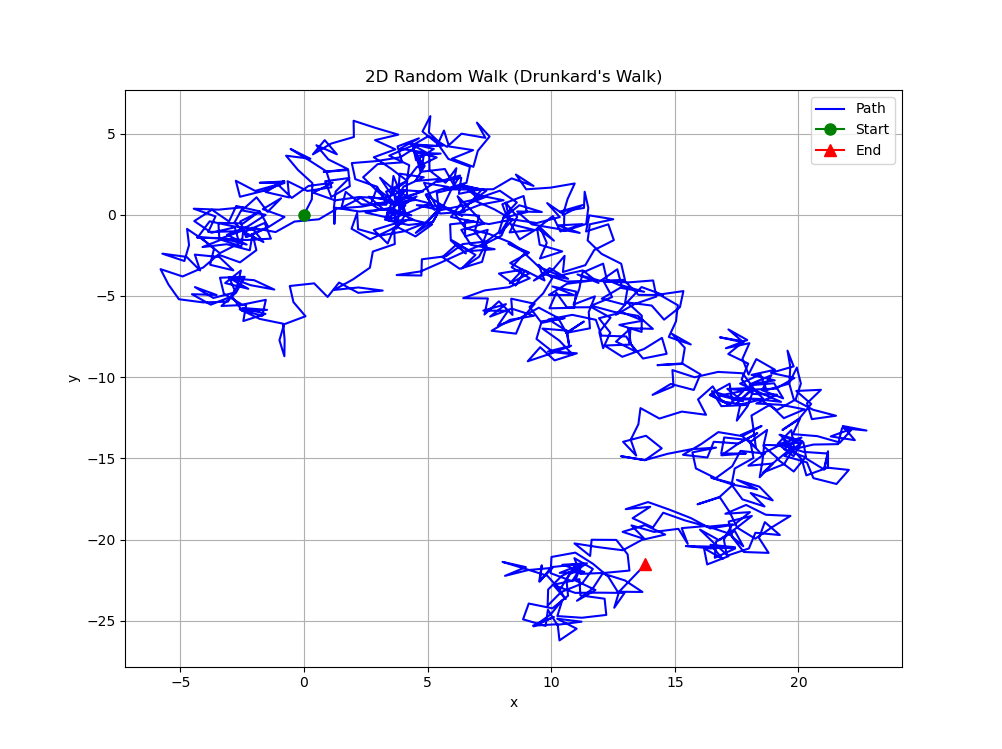
\includegraphics[width=0.6\textwidth]{images/problem_3_figure.png}
    \caption{Trajectory of a single "Drunkard's Walk" taking $T=1000$ steps in the 2D plane.}
    \label{fig:random_walk}
\end{figure}


\vspace{5cm}

\newpage
% ==========================================
% APPENDIX
% ==========================================
\appendix

\section{Terminal Output (Problem 2)}
Below is the exact, unedited terminal output from the Monte Carlo simulation (Problem 2).

\begin{outputbox}{Terminal Output: Problem 2 Results}
    ==========================
Running Problem 2: Estimating Pi
==========================

Running Problem 2a: Single Simulation for Each N
N: 10 Estimated Pi: 3.2
N: 100 Estimated Pi: 3.08
N: 1000 Estimated Pi: 3.152
N: 10000 Estimated Pi: 3.132
N: 100000 Estimated Pi: 3.14444
N: 1000000 Estimated Pi: 3.14356
N: 10000000 Estimated Pi: 3.14065

Running Problem 2b: 10 Simulations for Each N and Averaging
========================
N = 10
Run 1 | Pi Estimate: 2.4
Run 2 | Pi Estimate: 4
Run 3 | Pi Estimate: 3.6
Run 4 | Pi Estimate: 2.4
Run 5 | Pi Estimate: 2.4
Run 6 | Pi Estimate: 2.8
Run 7 | Pi Estimate: 3.2
Run 8 | Pi Estimate: 3.2
Run 9 | Pi Estimate: 3.6
Run 10 | Pi Estimate: 3.6
Average Pi for N = 10 : 3.12
========================
N = 100
Run 1 | Pi Estimate: 3.04
Run 2 | Pi Estimate: 3.08
Run 3 | Pi Estimate: 3.12
Run 4 | Pi Estimate: 3.08
Run 5 | Pi Estimate: 3.56
Run 6 | Pi Estimate: 3.12
Run 7 | Pi Estimate: 3.08
Run 8 | Pi Estimate: 3.12
Run 9 | Pi Estimate: 2.88
Run 10 | Pi Estimate: 3.2
Average Pi for N = 100 : 3.128
========================
N = 1000
Run 1 | Pi Estimate: 3.128
Run 2 | Pi Estimate: 3.088
Run 3 | Pi Estimate: 3.172
Run 4 | Pi Estimate: 3.096
Run 5 | Pi Estimate: 3.072
Run 6 | Pi Estimate: 3.16
Run 7 | Pi Estimate: 3.16
Run 8 | Pi Estimate: 3.036
Run 9 | Pi Estimate: 3.112
Run 10 | Pi Estimate: 3.088
Average Pi for N = 1000 : 3.1112
========================
N = 10000
Run 1 | Pi Estimate: 3.132
Run 2 | Pi Estimate: 3.1364
Run 3 | Pi Estimate: 3.1396
Run 4 | Pi Estimate: 3.1404
Run 5 | Pi Estimate: 3.1808
Run 6 | Pi Estimate: 3.1588
Run 7 | Pi Estimate: 3.1392
Run 8 | Pi Estimate: 3.1272
Run 9 | Pi Estimate: 3.154
Run 10 | Pi Estimate: 3.1412
Average Pi for N = 10000 : 3.14496
========================
N = 100000
Run 1 | Pi Estimate: 3.1298
Run 2 | Pi Estimate: 3.13788
Run 3 | Pi Estimate: 3.13864
Run 4 | Pi Estimate: 3.14596
Run 5 | Pi Estimate: 3.14484
Run 6 | Pi Estimate: 3.14304
Run 7 | Pi Estimate: 3.14096
Run 8 | Pi Estimate: 3.13984
Run 9 | Pi Estimate: 3.14184
Run 10 | Pi Estimate: 3.14552
Average Pi for N = 100000 : 3.14083
========================
N = 1000000
Run 1 | Pi Estimate: 3.14027
Run 2 | Pi Estimate: 3.13965
Run 3 | Pi Estimate: 3.14363
Run 4 | Pi Estimate: 3.14277
Run 5 | Pi Estimate: 3.13857
Run 6 | Pi Estimate: 3.14215
Run 7 | Pi Estimate: 3.1449
Run 8 | Pi Estimate: 3.13895
Run 9 | Pi Estimate: 3.14418
Run 10 | Pi Estimate: 3.1389
Average Pi for N = 1000000 : 3.1414
========================
N = 10000000
Run 1 | Pi Estimate: 3.14225
Run 2 | Pi Estimate: 3.1422
Run 3 | Pi Estimate: 3.14075
Run 4 | Pi Estimate: 3.14043
Run 5 | Pi Estimate: 3.14217
Run 6 | Pi Estimate: 3.14189
Run 7 | Pi Estimate: 3.14155
Run 8 | Pi Estimate: 3.1407
Run 9 | Pi Estimate: 3.14203
Run 10 | Pi Estimate: 3.14102
Average Pi for N = 10000000 : 3.1415

Running Problem 2c: Error Analysis
==============================
N = 10
Run 1 | Pi Estimate: 3.6 | Absolute Error: 0.458407
Run 2 | Pi Estimate: 3.2 | Absolute Error: 0.0584073
Run 3 | Pi Estimate: 3.6 | Absolute Error: 0.458407
Run 4 | Pi Estimate: 2.4 | Absolute Error: 0.741593
Run 5 | Pi Estimate: 4 | Absolute Error: 0.858407
Run 6 | Pi Estimate: 2.8 | Absolute Error: 0.341593
Run 7 | Pi Estimate: 3.2 | Absolute Error: 0.0584073
Run 8 | Pi Estimate: 3.6 | Absolute Error: 0.458407
Run 9 | Pi Estimate: 3.2 | Absolute Error: 0.0584073
Run 10 | Pi Estimate: 3.2 | Absolute Error: 0.0584073
Average Absolute Error for N = 10 : 0.355044
==============================
N = 100
Run 1 | Pi Estimate: 3.12 | Absolute Error: 0.0215927
Run 2 | Pi Estimate: 3.16 | Absolute Error: 0.0184073
Run 3 | Pi Estimate: 3.36 | Absolute Error: 0.218407
Run 4 | Pi Estimate: 3.28 | Absolute Error: 0.138407
Run 5 | Pi Estimate: 3.32 | Absolute Error: 0.178407
Run 6 | Pi Estimate: 3 | Absolute Error: 0.141593
Run 7 | Pi Estimate: 3.08 | Absolute Error: 0.0615927
Run 8 | Pi Estimate: 3.44 | Absolute Error: 0.298407
Run 9 | Pi Estimate: 3.16 | Absolute Error: 0.0184073
Run 10 | Pi Estimate: 3.08 | Absolute Error: 0.0615927
Average Absolute Error for N = 100 : 0.115681
==============================
N = 1000
Run 1 | Pi Estimate: 3.228 | Absolute Error: 0.0864073
Run 2 | Pi Estimate: 3.064 | Absolute Error: 0.0775927
Run 3 | Pi Estimate: 3.196 | Absolute Error: 0.0544073
Run 4 | Pi Estimate: 3.124 | Absolute Error: 0.0175927
Run 5 | Pi Estimate: 3.164 | Absolute Error: 0.0224073
Run 6 | Pi Estimate: 3.156 | Absolute Error: 0.0144073
Run 7 | Pi Estimate: 3.184 | Absolute Error: 0.0424073
Run 8 | Pi Estimate: 3.156 | Absolute Error: 0.0144073
Run 9 | Pi Estimate: 3.092 | Absolute Error: 0.0495927
Run 10 | Pi Estimate: 3.204 | Absolute Error: 0.0624073
Average Absolute Error for N = 1000 : 0.0441629
==============================
N = 10000
Run 1 | Pi Estimate: 3.1492 | Absolute Error: 0.00760735
Run 2 | Pi Estimate: 3.1412 | Absolute Error: 0.000392654
Run 3 | Pi Estimate: 3.1404 | Absolute Error: 0.00119265
Run 4 | Pi Estimate: 3.1444 | Absolute Error: 0.00280735
Run 5 | Pi Estimate: 3.1472 | Absolute Error: 0.00560735
Run 6 | Pi Estimate: 3.1664 | Absolute Error: 0.0248073
Run 7 | Pi Estimate: 3.1232 | Absolute Error: 0.0183927
Run 8 | Pi Estimate: 3.1212 | Absolute Error: 0.0203927
Run 9 | Pi Estimate: 3.1488 | Absolute Error: 0.00720735
Run 10 | Pi Estimate: 3.1272 | Absolute Error: 0.0143927
Average Absolute Error for N = 10000 : 0.01028
==============================
N = 100000
Run 1 | Pi Estimate: 3.1384 | Absolute Error: 0.00319265
Run 2 | Pi Estimate: 3.1376 | Absolute Error: 0.00399265
Run 3 | Pi Estimate: 3.14388 | Absolute Error: 0.00228735
Run 4 | Pi Estimate: 3.14072 | Absolute Error: 0.000872654
Run 5 | Pi Estimate: 3.1358 | Absolute Error: 0.00579265
Run 6 | Pi Estimate: 3.14152 | Absolute Error: 7.26536e-05
Run 7 | Pi Estimate: 3.13352 | Absolute Error: 0.00807265
Run 8 | Pi Estimate: 3.12964 | Absolute Error: 0.0119527
Run 9 | Pi Estimate: 3.13884 | Absolute Error: 0.00275265
Run 10 | Pi Estimate: 3.13528 | Absolute Error: 0.00631265
Average Absolute Error for N = 100000 : 0.00453012
==============================
N = 1000000
Run 1 | Pi Estimate: 3.14423 | Absolute Error: 0.00263535
Run 2 | Pi Estimate: 3.1412 | Absolute Error: 0.000396654
Run 3 | Pi Estimate: 3.14229 | Absolute Error: 0.000695346
Run 4 | Pi Estimate: 3.13907 | Absolute Error: 0.00252065
Run 5 | Pi Estimate: 3.14018 | Absolute Error: 0.00141265
Run 6 | Pi Estimate: 3.14418 | Absolute Error: 0.00258735
Run 7 | Pi Estimate: 3.14132 | Absolute Error: 0.000276654
Run 8 | Pi Estimate: 3.14001 | Absolute Error: 0.00158065
Run 9 | Pi Estimate: 3.13995 | Absolute Error: 0.00164065
Run 10 | Pi Estimate: 3.14165 | Absolute Error: 5.53464e-05
Average Absolute Error for N = 1000000 : 0.00138013
==============================
N = 10000000
Run 1 | Pi Estimate: 3.14149 | Absolute Error: 0.000100654
Run 2 | Pi Estimate: 3.14085 | Absolute Error: 0.000744654
Run 3 | Pi Estimate: 3.14088 | Absolute Error: 0.000713454
Run 4 | Pi Estimate: 3.14159 | Absolute Error: 5.85359e-06
Run 5 | Pi Estimate: 3.14127 | Absolute Error: 0.000324254
Run 6 | Pi Estimate: 3.14205 | Absolute Error: 0.000459346
Run 7 | Pi Estimate: 3.1419 | Absolute Error: 0.000302946
Run 8 | Pi Estimate: 3.1409 | Absolute Error: 0.000691454
Run 9 | Pi Estimate: 3.14238 | Absolute Error: 0.000782946
Run 10 | Pi Estimate: 3.14166 | Absolute Error: 6.37464e-05
Average Absolute Error for N = 10000000 : 0.000418931
\end{outputbox}

\newpage    

\section{Python Script for Plotting (Problem 2)}
Below is the Python script utilized to map the experimental data against the theoretical slope of $-0.5$ on a base-10 logarithmic scale.

\lstdefinestyle{pythonstyle}{
    language=Python,
    basicstyle=\ttfamily\scriptsize, 
    keywordstyle=\color{blue!80!black}\bfseries,
    stringstyle=\color{green!60!black},
    commentstyle=\color{gray}\itshape,
    showstringspaces=false,
    numbers=left,
    numberstyle=\tiny\color{gray},
    numbersep=3.5pt, % Adjust this value to move the line numbers left or right   breaklines=true,
    breaklines=true,
    tabsize=4
}
\newtcblisting{pythonbox}[1]{
    arc=3mm,
    boxrule=1pt,
    colback=yellow!5!white,
    colframe=yellow!50!black,
    title={\textbf{#1}},
    listing only,
    listing style=pythonstyle,
    breakable
}
\begin{pythonbox}{Python Source Code}
import numpy as np
import matplotlib.pyplot as plt
N = np.array([10, 100, 1000, 10000, 100000, 1000000, 10000000])
error = np.array([0.355044, 0.115681, 0.0441629, 0.01028, 0.00453012, 0.00138013, 0.000418931])

log_N = np.log10(N)
log_error = np.log10(error)

C = log_error[0] + 0.5 * log_N[0]
theoretical_line = -0.5 * log_N + C

plt.figure(figsize=(8, 6))

plt.plot(log_N, log_error, 'bo-', label='Experimental Data', markersize=6, linewidth=2)

plt.plot(log_N, theoretical_line, 'r--', label='Theoretical Line (Slope = -0.5)', linewidth=2)

plt.xlabel(r'$\log_{10}(N)$', fontsize=14)
plt.ylabel(r'$\log_{10}(Error)$', fontsize=14)
plt.title('Log-Log Plot of Monte Carlo Error vs. Sample Size', fontsize=16)
plt.legend(fontsize=12)
plt.grid(True, which="both", linestyle="--", alpha=0.7)

plt.savefig('error_plot.png', dpi=300, bbox_inches='tight')
plt.show()
\end{pythonbox}




\newpage
% ==========================================
% Appendix C: Compilation and Usage Guide
% ==========================================
\section{Compilation and Usage Guide}

% Define a clean style for terminal commands (Markdown-like)
\newtcolorbox{shellbox}{
    arc=1mm,
    boxrule=0.5pt,
    colback=gray!10!white,
    colframe=gray!40!black,
    fontupper=\ttfamily\small,
    left=2mm, right=2mm, top=1mm, bottom=1mm
}

\subsection{Dependencies}
The C++ solution utilizes \texttt{matplotlib-cpp} for visualization. If \texttt{matplotlibcpp.h} is not present in your directory, it can be downloaded via terminal:

\textbf{Using wget:}
\begin{shellbox}
wget https://raw.githubusercontent.com/lava/matplotlib-cpp/master/matplotlibcpp.h
\end{shellbox}

\textbf{Using curl (Standard on macOS):}
\begin{shellbox}
curl -O https://raw.githubusercontent.com/lava/matplotlib-cpp/master/matplotlibcpp.h
\end{shellbox}

\subsection{Compilation and Execution}
To compile and run the code, use the commands below. Note that the binary is named \texttt{mc}. (Note: Adjust python3.10 to your specific version if needed)

\textbf{macOS Compilation:}
\begin{shellbox}
g++ mc.cpp -std=c++11 \$(python3-config --cflags) \$(python3-config --ldflags) -o mc
\end{shellbox}

\textbf{Linux Compilation:}
\begin{shellbox}
g++ mc.cpp -std=c++11 -I/usr/include/python3.10 -lpython3.10 -o mc
\end{shellbox}

\textbf{Run the Code:}
\begin{shellbox}
./mc
\end{shellbox}

\subsection{Nested Execution Control}
The code is designed with \textbf{nested modularity} to allow fine-grained control over which simulations are executed. 

\begin{enumerate}
    \item \textbf{High-Level Control:} In \texttt{main()}, you can comment out \texttt{run\_problem\_2()} or \texttt{run\_problem\_3()} to skip an entire problem set.
    \item \textbf{Sub-Task Control:} Inside the \texttt{run\_problem\_X()} wrapper functions, you can comment out specific sub-tasks (e.g., part (a), (b), or (c)) to focus only on a particular analysis.
\end{enumerate}

\begin{codebox}{Example: Toggling Sub-Tasks in Problem 2}
void run_problem_2 (){
    int N[] = {10, 100, 1000, 10000, 100000, 1000000, 10000000};
    int size = sizeof(N) / sizeof(N[0]);

    // Toggle specific sub-tasks here:
    // run_problem_2_a(N, size); 
    // run_problem_2_b(N, size, 10);
    run_problem_2_c(N, size); // Only part (c) will execute
}
\end{codebox}

\end{document}